\documentclass[onecolumn,10pt]{jhwhw}

\usepackage{epsfig} %% for loading postscript figures
\usepackage{amsmath}
\usepackage{graphicx}
\usepackage{grffile}
\usepackage{pdfpages}
\usepackage{algpseudocode}
\usepackage{wrapfig}
\usepackage{pgfplots}
\usepackage{amsfonts}
\usepackage{booktabs}
\usepackage{siunitx}
\usepackage{commath}
\usepackage{rotating}
\usepackage{url}
\usepackage{multimedia}
\usepackage{hyperref}
\usepackage{mathtools}

% Default fixed font does not support bold face
\DeclareFixedFont{\ttb}{T1}{txtt}{bx}{n}{12} % for bold
\DeclareFixedFont{\ttm}{T1}{txtt}{m}{n}{12}  % for normal

% Custom colors
\usepackage{color}
\usepackage{listings}
\usepackage{framed}
\usepackage{caption}
\usepackage{bm}
\captionsetup[lstlisting]{font={small,tt}}

\definecolor{mygreen}{rgb}{0,0.6,0}
\definecolor{mygray}{rgb}{0.5,0.5,0.5}
\definecolor{mymauve}{rgb}{0.58,0,0.82}

\lstset{ %
  backgroundcolor=\color{white},   % choose the background color; you must add \usepackage{color} or \usepackage{xcolor}
  basicstyle=\ttfamily\footnotesize, % the size of the fonts that are used for the code
  breakatwhitespace=false,         % sets if automatic breaks should only happen at whitespace
  breaklines=true,                 % sets automatic line breaking
  captionpos=b,                    % sets the caption-position to bottom
  commentstyle=\color{mygreen},    % comment style
  deletekeywords={...},            % if you want to delete keywords from the given language
  escapeinside={\%*}{*)},          % if you want to add LaTeX within your code
  extendedchars=true,              % lets you use non-ASCII characters; for 8-bits encodings only, does not work with UTF-8
  frame=single,                    % adds a frame around the code
  keepspaces=true,                 % keeps spaces in text, useful for keeping indentation of code (possibly needs columns=flexible)
  columns=flexible,
  keywordstyle=\color{blue},       % keyword style
  language=Python,                 % the language of the code
  morekeywords={*,...},            % if you want to add more keywords to the set
  numbers=left,                    % where to put the line-numbers; possible values are (none, left, right)
  numbersep=5pt,                   % how far the line-numbers are from the code
  numberstyle=\tiny\color{mygray}, % the style that is used for the line-numbers
  rulecolor=\color{black},         % if not set, the frame-color may be changed on line-breaks within not-black text (e.g. comments (green here))
  showspaces=false,                % show spaces everywhere adding particular underscores; it overrides 'showstringspaces'
  showstringspaces=false,          % underline spaces within strings only
  showtabs=false,                  % show tabs within strings adding particular underscores
  stepnumber=1,                    % the step between two line-numbers. If it's 1, each line will be numbered
  stringstyle=\color{mymauve},     % string literal style
  tabsize=4,                       % sets default tabsize to 2 spaces
}

\usepackage{etoolbox}
\renewcommand{\lstlistingname}{Diagram}% Listing -> Algorithm
\patchcmd{\thebibliography}{\chapter*}{\section*}{}{}

\author{John Karasinski}
\title{Homework 5}

\begin{document}
%\maketitle

\problem{}
\textit{Orbital Transfer Review: remind yourself: (discuss/justify decisions)} \\
\\
All three of the transfers below can be accomplished with a Hohmann transfer. The amount of $\Delta V$ required for a Hohmann transfer is
\begin{align*}
\Delta v_1 &= \sqrt{\dfrac{\mu}{r_1}} \left(\sqrt{\dfrac{2r_2}{r_1 + r_2}} -1 \right), \\
\Delta v_2 &= \sqrt{\dfrac{\mu}{r_2}} \left(1 - \sqrt{\dfrac{2r_1}{r_1 + r_2}} \right), \\
\Delta v_{total} &= \Delta v_1 + \Delta v_2.
\end{align*}
Additionally, part (b) requires an inclination change. The $\Delta V$ budget for a inclination change for a circular orbit is
\begin{align*}
\Delta{v_i}= 2 v \sin \left( \dfrac{\Delta i}{2} \right).
\end{align*}
The assumption of a circular orbit should be fine here, as both HST and ISS orbits have very low eccentricity.

\begin{enumerate}
\itemsep0em
\item Determine the $\Delta V$ required to move from a 200km coplanar parking orbit to the HST orbit
\begin{align*}
r_1 &= 200 km + 6,371 km \\
r_2 &= 569 km + 6,371 km \\
\Delta v_{total} &= \Delta v_{Hohmann} \\
                 &= 0.210 km/s.
\end{align*}
\item Determine the $\Delta V$ required to move from the ISS orbit to the HST orbit
\begin{align*}
r_{ISS} &= 414.1 km + 6,371 km \\
r_{HST} &= 569 km + 6,371 km \\
i_{ISS} &= 0.9014 rad \\
i_{HST} &= 0.4969 rad \\
v_{HST} &= 7.59 km/s \\
\\
\Delta v_{total} &= \Delta v_{Hohmann} + \Delta v_{Plane Change} \\
                 &= 0.086 + 3.049 \\
                 &= 3.135 km/s,
\end{align*}
where we've again assumed a circular orbit. The plane change should take place after the Hohmann transfer, as the orbital velocity is lower at HST orbit, leading to a smaller required $\Delta V$.

\item Determine the $\Delta V$ required to deorbit from the HST orbit (must choose your de-orbit orbital params)
\begin{align*}
r_{deorbit} &= 100 km + 6,371 km \\
r_{HST} &= 569 km + 6,371 km \\
\Delta v &= \sqrt{\dfrac{\mu}{r_1}} \left(\sqrt{\dfrac{2r_2}{r_1 + r_2}} -1 \right), \\
         &= 0.136 km/s,
\end{align*}
where a height of $100km$ should be sufficient to cause the vehicle to deorbit rapidly.
\end{enumerate}

\problem{}
\textit{Eclipse durations (text 5.3.2): an important design aspect of your solar array system is the relative durations of eclipse and insolation. Using the algorithm given in section 5.3.2,}
\begin{enumerate}
\itemsep0em
\item Compute the eclipse period for ISS, for HST, and for a typical GPS satellite (choose one)
\end{enumerate}

I ran the algorithm in section 5.3.2 over one complete orbit at 0.1 degree increments, and for sun positions of one complete year at day increments. The mean and standard error of the mean was calculated for eclipse period, as was the total time in eclipse and the total number of eclipses over the one year period. These results are presented in Table~\ref{p2table}.

\begin{table}[h]
\begin{center}
\begin{tabular}{rrrrr}
\toprule
Satellite & Mean (min) & SEM (min) & Total (hrs) & Count \\
\midrule
HST & 33.97 & 0.10 & 414.45 & 732 \\
ISS & 34.99 & 0.09 & 426.98 & 732 \\
GPS & 46.09 & 2.55 &  90.64 & 118 \\
\bottomrule
\end{tabular}
\end{center}
\caption{Eclipse statistics for the HST, ISS, and a GPS satellite (Navstar 43)}
\label{p2table}
\end{table}

\clearpage

\problem{}
\textit{Let’s say we lose control of your spacecraft after it has undocked from HST, but before it has de-orbited.}
\begin{enumerate}
\itemsep0em
\item Estimate the orbital lifetime of your spacecraft (text 5.3.4) following loss of communications: assume HST circular orbit, average solar activity.

The lifetime of an uncontrolled space vehicle is approximately
\begin{align*}
\tau &\sim \dfrac{e_0^2}{2B} \left( 1 - \dfrac{11}{6}e_0 + \dfrac{29}{16}e_0^2 + \dfrac{7}{8} \dfrac{H}{a_0} \right)
\end{align*}
where $e_0$ and $a_0$ are the initial values of eccentricity and semi-major axis once control has ceased, $H$ is the scale height of the atmosphere near perigee and $B$ is given by
\begin{align*}
B &\sim \sqrt{\dfrac{\mu}{a_o^3}} \dfrac{A C_D}{M} \rho_{p_0} a_0 e_0 I_1 \left( \dfrac{a_0 e_0}{H} \right) exp \left(-e_0 \left(1 + \dfrac{a_0}{H} \right) \right)
\end{align*}

Assuming a small $e \approx 0.0002468, C_D = 2.2, \rho \approx 6.5$E-13 kg/m$^3, H \approx 72500,$ m and $A = 16$m$^2$, we find a time, $\tau = 718.3$ days, or approximately 2 years.


\item Would it make any difference to the decay timescale whether your spacecraft was tumbling or not?

Tumbling has no affect on any of the parameters in $\tau$, except for the area, $A$. A tumbling craft would have a continuously changing $A$, which could increase or decrease the lifetime of the vehicle.
\end{enumerate}

\problem{}
\textit{Geostationary orbits (text 5.6):}
\begin{enumerate}
\itemsep0em
\item Using the linearized solution to Kepler’s equation given in eqns 5.27-5.29, plot ground-track fluctuations as longitude vs latitude. Describe the results.
\begin{figure}[tbh!]
\begin{center}
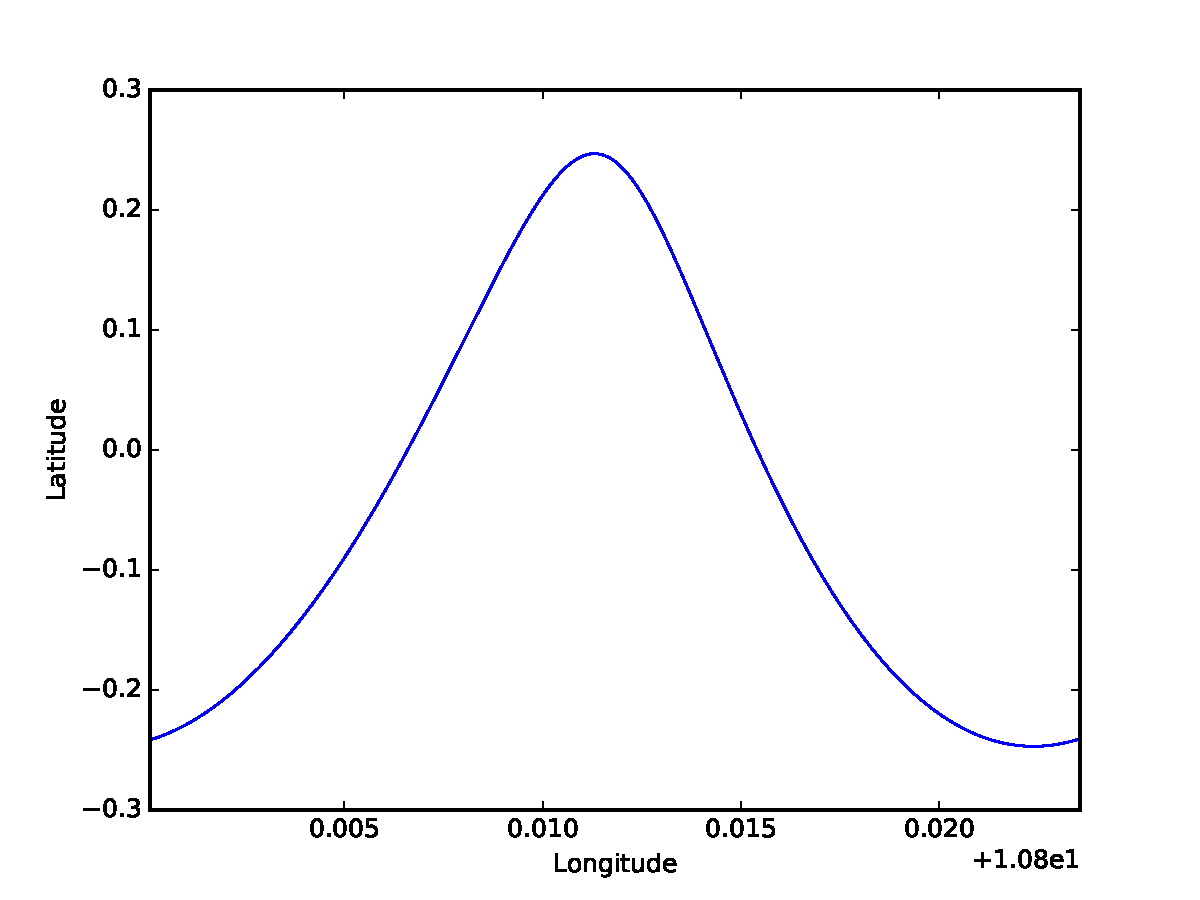
\includegraphics[height=0.45\textheight]{p4a-1.pdf}
% 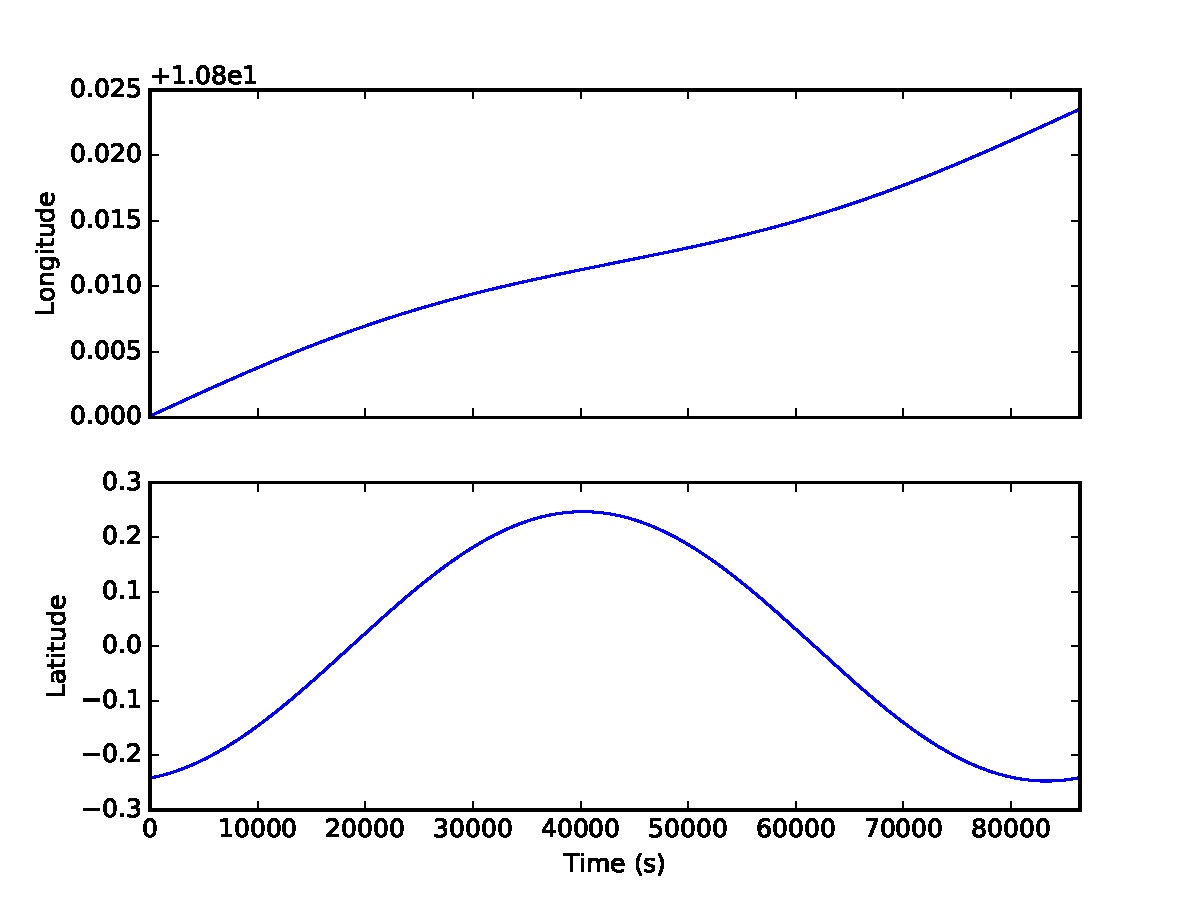
\includegraphics[height=0.45\textheight]{p4a-2.pdf}
\end{center}
\caption{Ground Track Fluctuations as Longitude vs Latitude}
\label{fig:gtf}
\end{figure}

The longitude and latitude can be calculated by
\begin{align*}
\lambda &= \Omega + \omega - \dfrac{3}{2} \dfrac{\delta a}{A} t \sqrt{\dfrac{\mu}{A^3}} + 2e\sin{\left(t \sqrt{\dfrac{mu}{A^3}} \right)} \\
\theta &= i \sin{\left( \omega + t \sqrt{\dfrac{mu}{A^3}} \right)}.
\end{align*}
Figure~\ref{fig:gtf} shows the Longitude and Latitude for Westar 1, America's first domestic and commercially launched geostationary communications satellite. Here $i = 14.15^o, \omega = 282^o, \Omega = 336.8^o, e=7.333$E-4, $A=42164.5$km, and $\delta a=42164.5 - 42269=-104.5$km. The groundtrack is shown here for 24 hours, which is roughly equivalent to one orbit. The latitudinal variation is a simple oscillation, while the longitudinal variations include an oscillation and a small drift rate from the small $\delta a$ value.


\item Define deadband and control limit-cycle in the context of GEO station keeping.

The dead band of a GEO satellite is the maximum allowable error in $\lambda$, and the control limit-cycle describes how often a burn is required in order to return this error to the opposite side of the dead band.

\item Consider a GEO satellite with nominal longitude of -100deg, and an onboard propellant system capable of providing a total $\Delta V$ of 200m/s. For a maximum longitudinal error magnitude of 0.22deg, for how long can the satellite station-keep?

The required $\Delta V$ required to keep the satellite within $\lambda_{max}$ degrees of error with a limit cycle of $T$ is
\begin{align*}
\Delta V =& 4 \sqrt{\dfrac{rf \lambda_{max}}{3}} = 0.083 \mbox{ m/s}\\
       T =& 4 \sqrt{\dfrac{r \lambda_{max}}{3f}} = 0.326 \mbox{ years},
\end{align*}
where $f = +8.10$ E-9 m/s$^2$, $\lambda_{max} = 0.22$ deg, and $r = 42E6$ m. The length of time a satellite can station keep with fuel $\Delta V_{total}$ is then
\begin{align*}
T_{station keep} &= \Delta V_{total} / \left( \dfrac{\Delta V}{T} \right) = 782.957 \mbox{ years},
\end{align*}
which simply means that the lognitudinal station keeping is not the limiting factor of the satellite's lifespan.
\end{enumerate}

\problem{}
\textit{Two spacecraft in elliptical Earth orbit with the orbital parameters as follows. Compute the relative position and velocity vectors.}
\begin{enumerate}
\itemsep0em
\item h= 52,059 km$^2$/s, e=0.0257240, i=60deg, $\Omega$=40deg, $\omega$=30deg, $\theta$=40deg
\item h= 52,362 km$^2$/s, e=0.0072696, i=50deg, $\Omega$=40deg, $\omega$=120deg, $\theta$=40deg
\end{enumerate}

We can calculate the Earth-centric position and velocity vectors with the \verb|sv_from_coe()| function developed in Homework 4. They are
\begin{enumerate}
\itemsep0em
\item $[\textbf{r}_1 \textbf{ v}_1] = [-266.7,  3865.7,  5426.1, -6.4 , -3.6,  2.4]$
\item $[\textbf{r}_2 \textbf{ v}_2] = [-5890.7, -2979.7,  1792.2, 0.9, -5.2, -5.5]$,
\end{enumerate}
Where \textbf{r} is in km, and \textbf{v} is in km/s. To calculate \textbf{r} we can simply take the difference
\begin{align*}
   \textbf{r}_{rel} &= \textbf{r}_2 - \textbf{r}_1 \\
                    &= [-5623.9, -6845.5, -3633.9] \mbox{ km}
\end{align*}

The relative velocity vector can be caluclated by
\begin{align*}
\textbf{v}_{2} &= \textbf{v}_1 + \textbf{$\Omega$} \times \textbf{r}_{rel} + \textbf{v}_{rel},
\end{align*}
where
\begin{align*}
\textbf{$\Omega$} &= \dfrac{\textbf{r} \times \textbf{v}}{\textbf{r}^2} \\
 &= \left|
 \begin{array}{ccc}
 i & j & k \\
 -266.7 & 3865.7 & 5426.1 \\
 -6.4 & -3.6 &  2.4 \\
 \end{array}
 \right| \cdot \dfrac{1}{(6667.7)^2} \\
 &= \dfrac{28979.7i -34536.6j + 26029.5k}{(6667.7)^2} \\
 &= [ 0.00065, -0.00077,  0.00058] \mbox{ rad/s}
\end{align*}
Rearranging, we have,
\begin{align*}
\textbf{v}_{rel} &= \textbf{v}_{2} - \textbf{v}_1 - \textbf{$\Omega$} \times \textbf{r}_{rel} \\
\phantom{\textbf{v}_{rel}} &= [0.9, -5.2, -5.5] - [-6.4, -3.6, 2.4] - \left|
 \begin{array}{ccc}
 i & j & k \\
 0.00065 & -0.00077 & 0.00058 \\
 -5623.9 &  -6845.5 & -3633.9 \\
 \end{array}
 \right| \\
\textbf{v}_{rel} &= [0.58855, -0.69663,  0.91435] \mbox{ km/s}.
\end{align*}

\clearpage

\problem{}
\textit{Fly-around relative trajectories: for the lost EVA toolbox example considered in lecture, generate the relative motion plot for 1 orbital period, given initial conditions of:}
\begin{enumerate}
\itemsep0em
\item Release relative velocity = (-0.1, 0, 0) m/s (prolate cycloid)
\begin{figure}[h!]
\begin{center}
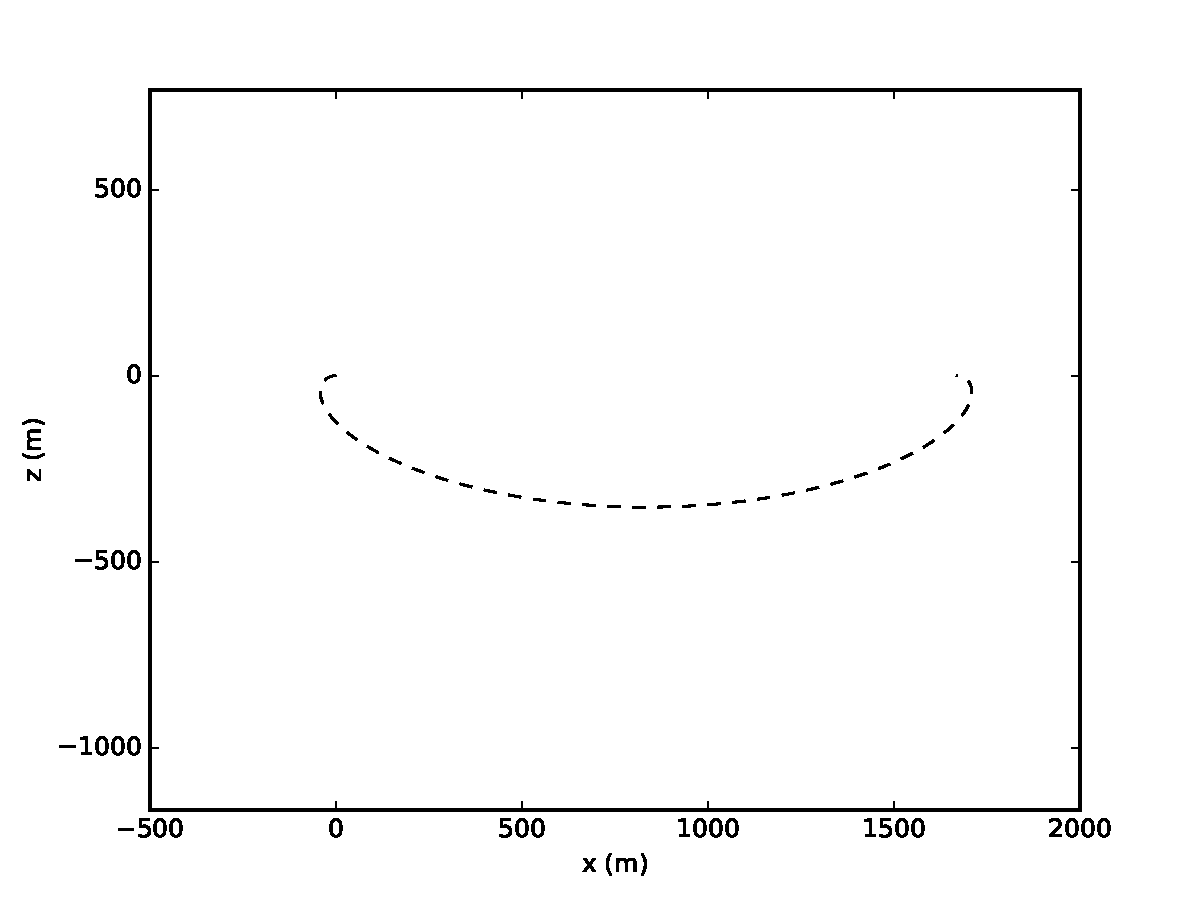
\includegraphics[height=0.37\textheight]{6a.pdf}
\end{center}
\end{figure}
\item Release relative velocity = (0, 0, 0.1) m/s (ellipse)
\begin{figure}[h!]
\begin{center}
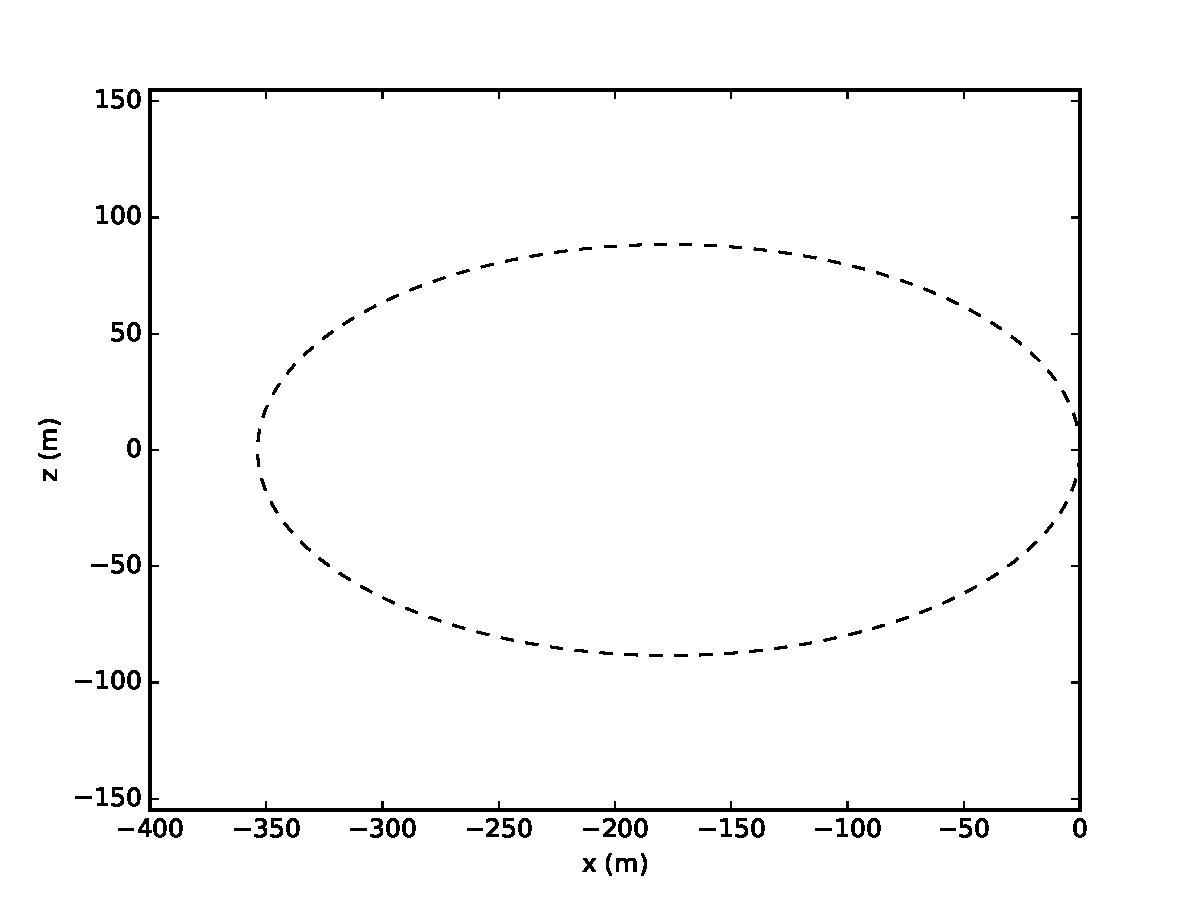
\includegraphics[height=0.37\textheight]{6b.pdf}
\end{center}
\end{figure}
\item Release relative velocity = (-0.1, 0, 0.1) m/s (initially 45deg backwards and up; describe subsequent motion)
\begin{figure}[h!]
\begin{center}
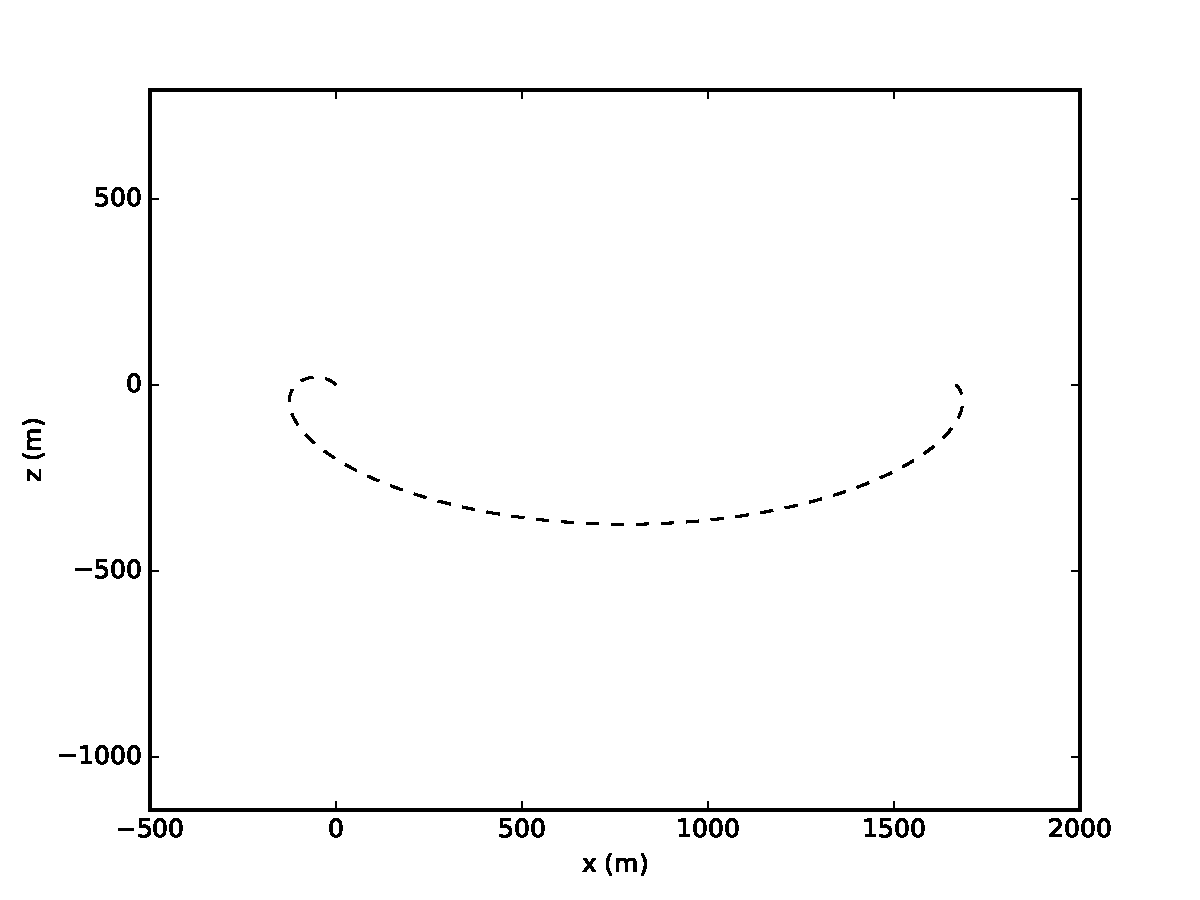
\includegraphics[height=0.3\textheight]{6c.pdf}
\end{center}
\vspace{-1.5em}
\end{figure}

This motion looks very similar to the prolate cycloid, except that altitude is gained during the very beginning of the orbit.
\item For a and b, plot the trajectory with and without the nt$\ll$1 assumption. Discuss.
\begin{figure}[h!]
\begin{center}
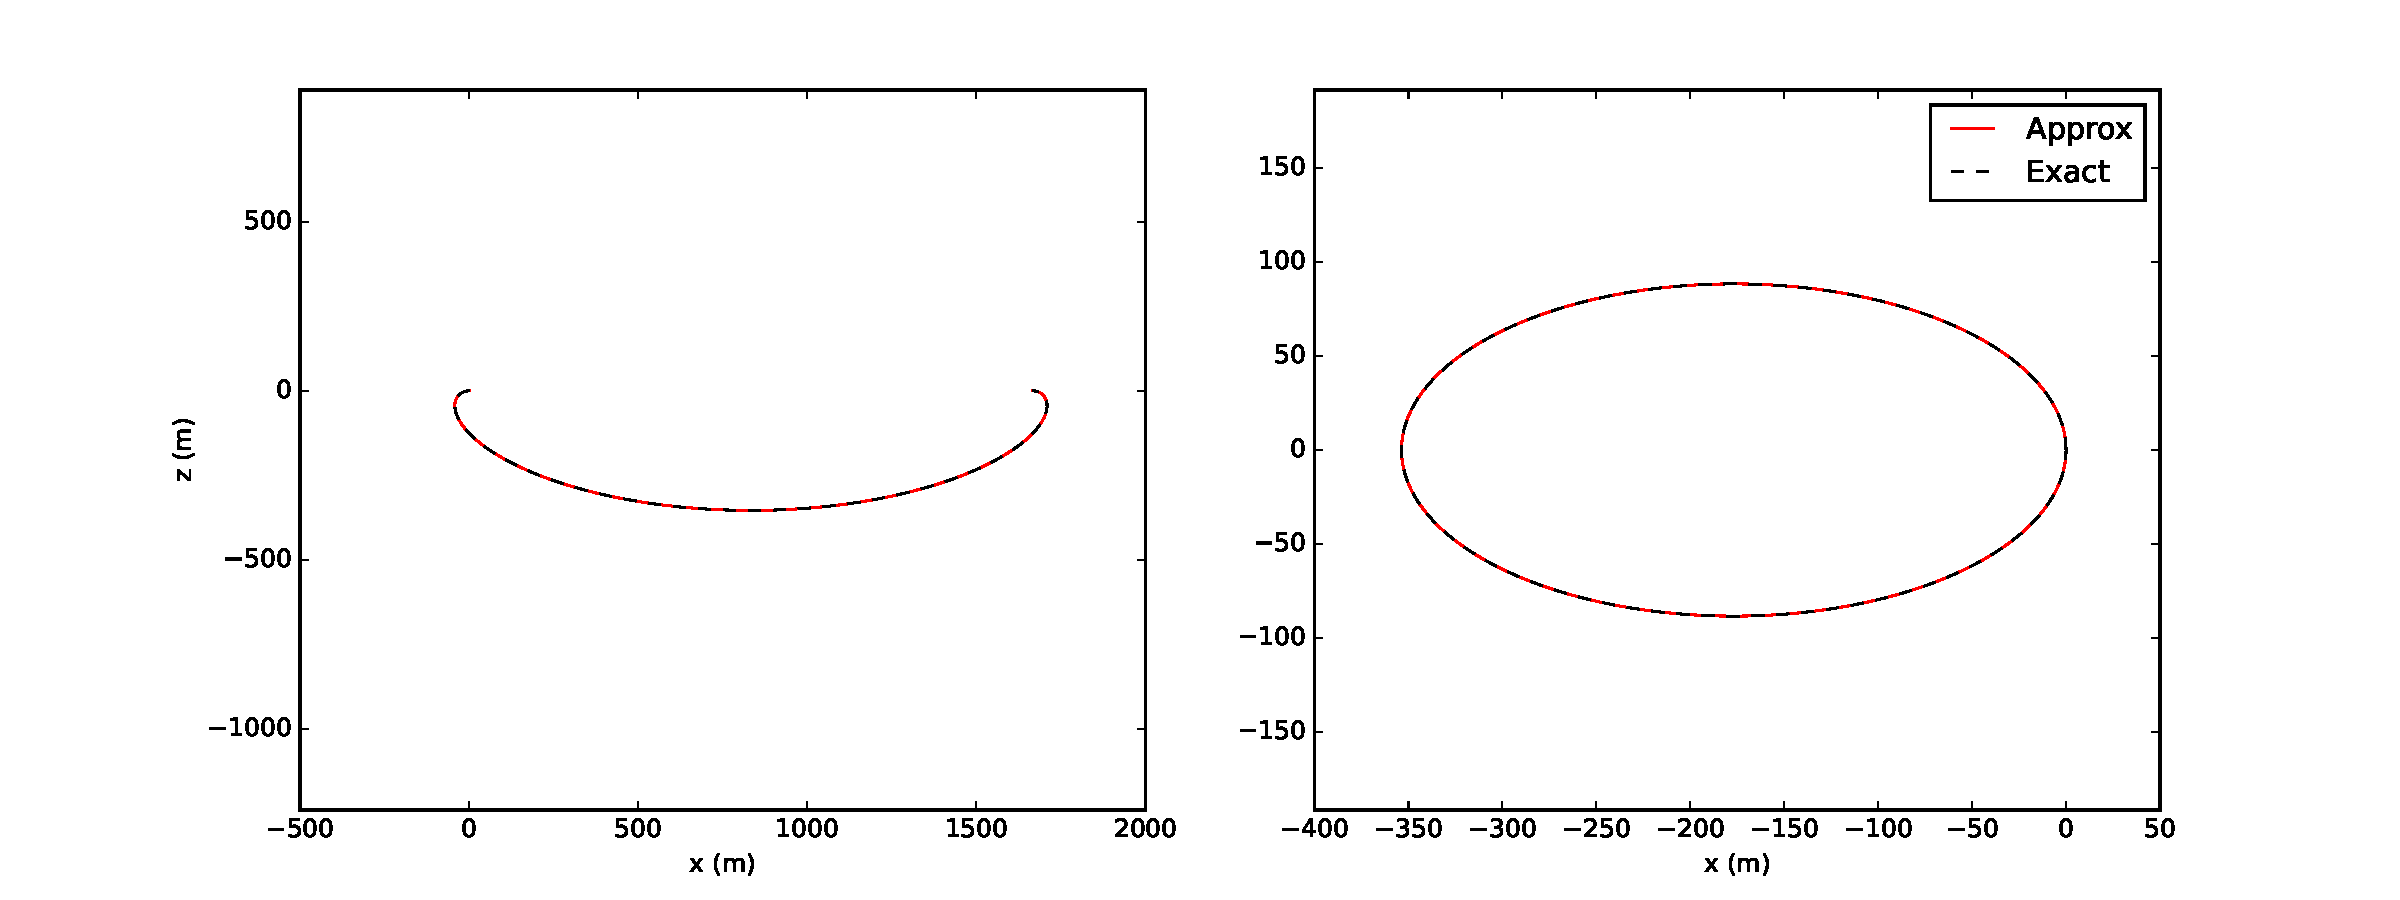
\includegraphics[width=1\textwidth]{6dboth.pdf}
\end{center}
\vspace{-1.5em}
\end{figure}

The $\cos$ and $\sin$ parts of the solution were expanded to their first two Taylor series components. Compared to the exact solutions, these approximate solutions performed very well. There is a minimal difference between the two solutions for one orbit.
\item How about a release relative velocity = (0, 0.1, 0) m/s? Would you see the toolbox again or not?

Motion along the y axis simply acts as a harmonic oscillator. If the orbit was sufficiently high enough, so that drag and and other orbit perturbations were minimal, you may indeed see the toolbox again. For ISS orbit, however, drag would dominate, and you would not see the toolbox again.
\end{enumerate}
\clearpage

\problem{}
\textit{For your HST re-boost spacecraft, assume:}
\begin{itemize}
\itemsep0em
\item[--] Launch: drop-off circular orbit at 200km, in-plane with HST, 65deg phase angle behind HST
\item[--] Phasing: 4-orbit phasing to point S1, 30km behind and 10km below HST
\item[--] Homing: Hohmann S1 to co-orbit waiting point S2, 1km behind HST
\item[--] Closing: Cycloid close waiting point S3, 200m behind HST
\end{itemize}
\begin{enumerate}
\itemsep0em
\item compute the required $\Delta V$ and elapsed time for each phase, and for the total rendezvous to S3

To get to approximately 30km and 10km below HST, we need to phase our orbits. The amount of change in phase after each orbit is
\begin{align*}
\Delta \theta &= -3 \pi \dfrac{\Delta a}{a} \\
              &= -3 \pi \dfrac{550 \mbox{ km} - 200 \mbox{ km}}{550 \mbox{ km} + 6371 \mbox{ km}} \\
              &= -27.3 \mbox{ degree},
\end{align*}
so we'll begin our homing phase after two orbits. For the homing burn, we will burn from $\Delta a = -10$km to a waiting point $S1 = 1$km behind the HST. We have $\theta_f = (180^o/\pi) \cdot (10/6921) = 0.0827^o$ and $v_T = 7.591$ km s$^{-1}$. With this we get $\theta_i = \theta_f + .195^o = .278^o$. $2 \pi(\frac{0.278^o}{360^o}) \cdot 6921 = 33.58$ km, which is approximately 30km. This means we have to perform a burn with
\begin{align*}
\Delta v &= - \dfrac{1}{2}\dfrac{\Delta a}{a}\sqrt{\dfrac{\mu}{a}} \\
         &= 5.482 \mbox{ m/s},
\end{align*}
which will take a time, $t_H$, of
\begin{align*}
t_H &= \pi \sqrt{\dfrac{a_H^3}{\mu}} \\
    &= \pi \sqrt{\dfrac{\left( a \left[ 1 + \dfrac{\Delta a}{2a} \right] \right)^3}{\mu}} \\
    &= 2862.0 \mbox{ s}.
\end{align*}
We use a cycloidal approach to close, with a total $\Delta v$ requirement of
\begin{align*}
\Delta v &= 2 \times \dfrac{\Delta x}{6 \pi \cdot k} \sqrt{\dfrac{\mu}{a^3}}\\
         &= 0.093 \mbox{ m/s},
\end{align*}
where $\Delta x = 800$ m. Here $k=1$ has been chosen to minimize the required time to approach. This will take one full orbital period, for a total time of 5728.8 seconds. \\
\\
This brings the total $\Delta v$ requirements to 5.575 m/s, and the total time to 20048.4 seconds, or 3.5 orbits.
\begin{table}[h]
\begin{center}
\begin{tabular}{rrr}
\toprule
Phase    & $\Delta V$ & Time (s) \\
\midrule
Phasing & - & 11457.6 \\
Homing & 5.482 & 2862.0 \\
Closing & 0.093 & 5728.8 \\
\midrule
Total & 5.575 & 20048.4\\
\bottomrule
\end{tabular}
\end{center}
\caption{$\Delta V$ and time requirements for each phase of rendezvous}
\end{table}

\item compute the view-angle to HST, measured from the orbit-tangent (for sensor acquisition)

The view-angle is simply calculated by
\begin{align*}
\theta &= \arctan{\left(\frac{10 \mbox{ km}}{30 \mbox{ km}} \right)} \\
       &= 18.43^o
\end{align*}
\item plot the total quantitative relative motion (like Walter Fig. 8.26)
\end{enumerate}

\end{document}
